\section{Introduzione}
\subsection{Problemi}
Per descrivere un \g{problema} bisogna specificare:
\begin{itemize}
	\item  Insieme dei possibili Input
	\item  Insieme dei possibili Output
	\item  La relazione tra Input e Output
\end{itemize}
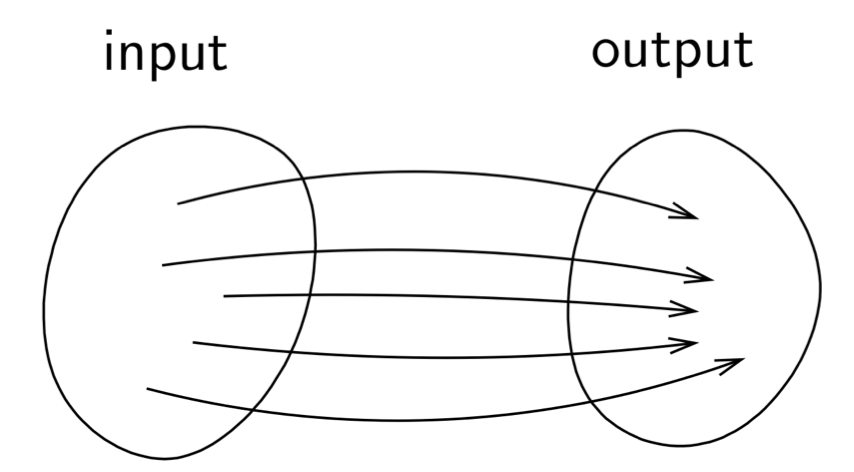
\includegraphics[scale=0.5]{img/funzione.png}

\nin\g{Algoritmo}: procedura meccanica che esegue delle computazioni (e può essere eseguita da un calcolatore).\\
Un algoritmo \g{risolve} un dato problema se:
\begin{itemize}
	\item Per ogni input, il calcolo dell'algoritmo si interrompe dopo un numero finito di passaggi.
	\item Per ogni input, l'algoritmo produce un output corretto.
\end{itemize}
\g{Correttezza} di un algoritmo:
Verificare che l'algoritmo risolva realmente il problema dato\\
\g{Complessità computazionale} di un algoritmo:
\begin{itemize}
	\item  \g{complessità temporale}: come varia il tempo di esecuzione rispetto alla dimensione dei dati di input
	\item  \g{complessità spaziale}: come varia la quantità di memoria utilizzata rispetto alla dimensione dei dati di input
\end{itemize}
\subsection{Linguaggi Formali}
\begin{itemize}
	\item Astrazione della nozione di problema
	\item I problemi sono espressi come \g{linguaggi} (insieme di stringhe) 
	\item Le soluzioni determinano se una determinata stringa è nell'insieme o no
		\begin{itemize}
			\item  Esempio: \textit{un certo intero $n$ è un numero primo?}
		\end{itemize}
	\item  Oppure, come \textit{trasformazioni tra linguaggi}
		\begin{itemize}
			\item Le soluzioni trasformano la stringa di input in una stringa di output
				\begin{itemize}
					\item Esempio: \textit{quanto fa $3+5$?}
				\end{itemize}
		\end{itemize}
\end{itemize}
Quindi in sostanza tutti i processi computazionali possono essere ridotti ad uno tra:
\begin{itemize}
	\item Determinazione dell'\textit{appartenenza} a un insieme (di stringhe)
	\item \textit{Mappatura} tra insiemi (di stringhe)
\end{itemize}
Formalizzeremo il concetto di computazione meccanica:
\begin{itemize}
	\item Dando una definizione precisa del termine "algoritmo"
	\item Caratterizzando i problemi che sono o non sono adatti per essere risolti da un calcolatore
\end{itemize}
\subsection{Automi}
Gli \textit{automi} sono dispositivi matematici astratti che possono:
\begin{itemize}
	\item Determinare l'appartenenza di una stringa ad un insieme di stringhe
	\item Trasformare una stringa in un'altra stringa
\end{itemize}
Hanno tutti gli \textit{aspetti} di un computer\\
Il tipo di \g{memoria} è cruciale:
\begin{itemize}
	\item memoria finita
	\item memoria infinita:
		\begin{itemize}
			\item con accesso limitato
			\item con accesso illimitato
		\end{itemize}
\end{itemize}
Abbiamo diversi tipi di automi per diversi classi di linguaggi\\
I diversi tipi di automi si differenziano per
\begin{itemize}
	\item La quantità di memoria (finita vs infinita)
	\item Il tipo di accesso alla memoria (limitato vs illimitato)
\end{itemize}
